The given equation can be expressed as 
\begin{align}
\norm{\vec{x}}^2+2\myvec{\frac{-1}{4} & 0}\vec{x}&=0
\end{align}	
The centre of circle is then given by 
\begin{align}
	\vec{u} = -\vec{c} 
=\myvec{\frac{1}{4}\\0}
\end{align}
and the radius of circle is obtained as
\begin{align}
	r=\sqrt{\norm{\vec{u}}^2 -f}
=\frac{1}{4}
\end{align}
\iffalse
See 
  \figref{fig:chapters/11/11/1/9/Figure}.
\begin{figure}[H]
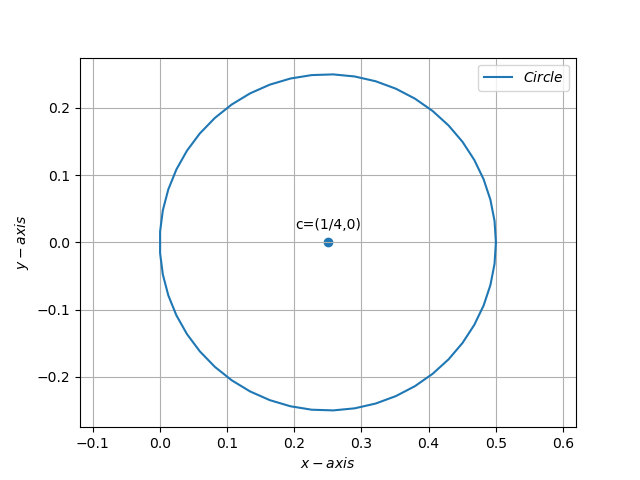
\includegraphics[width=0.75\columnwidth]{chapters/11/11/1/9/figs/fig.png}
\caption{}
  \label{fig:chapters/11/11/1/9/Figure}
\end{figure}
\fi
